\documentclass[10pt]{beamer}

\usetheme{metropolis}
\usepackage{appendixnumberbeamer}
\usepackage[utf8]{inputenc}
\usepackage[russian,francais]{babel}
\usepackage{booktabs}
\usepackage[scale=2]{ccicons}
\usepackage{pdfpages}
\usepackage{pgfplots}
\usepgfplotslibrary{dateplot}
\usepackage{subcaption}
\usepackage{amsmath, amssymb}
\usepackage{booktabs}
\usepackage{graphicx}
\usepackage{hyperref}
\usepackage{xspace}
\usepackage{listings}
\usepackage{diagbox}

% Python for inline
\newcommand\pythoninline[1]{{\pythonstyle\lstinline!#1!}}
%%\usepackage{polyglossia}
%%    \setdefaultlanguage{french} % main language
%%    \setotherlanguages{russian, hindi, greek, hebrew} % other languages 
%%\graphicspath{{images/}}	% Put all images in this directory. Avoids clutter.
%%\setmainfont{Latin Modern Roman}
%%\setsansfont{Latin Modern Sans}
%%\setmonofont{Latin Modern Mono}
%%\setmainfont[Ligatures=TeX]{Times New Roman}
%%\newfontfamily{\cyrillicfonttt}{Times New Roman}[Script=Cyrillic]

\title{M3SOL025 - Diagnostic de Langue}
\date{2025-2026}
\author{Gaël Lejeune \quad {gael.lejeune@sorbonne-universite.fr}}
\institute{STIH EA 4509, CERES, Sorbonne Université}
 \titlegraphic{\hfill
\includegraphics[height=.7cm]{../images/sorbon.png}}
\begin{document}
\maketitle

%%\begin{frame}{Plan de la présentation}
%%  \setbeamertemplate{section in toc}[sections numbered]
%%  \tableofcontents[hideallsubsections]
%%\end{frame}

%Matrice confusion langid et BAseline
% quelle est cette langue "la" ? cf tableau d'AMina et Heatmap de Camille
% Description corpus taille
% Scale et dopesick
\section{Contextualiser les données}
\begin{frame}{Stocker les résultats : bonne idée}

\begin{figure}
  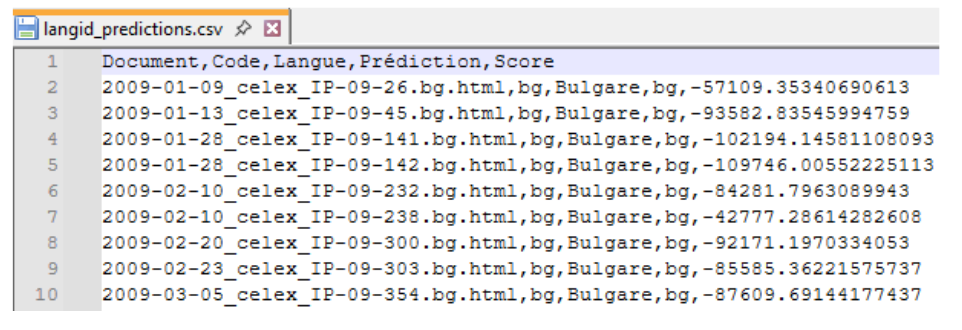
\includegraphics[width=.8\textwidth]{images/Stocker.png}
  \caption{Evaluation Online VS Offline ?}
\end{figure}
\end{frame}

\begin{frame}{Observer indépendamment des résultats : bonne idée}

\begin{figure}
  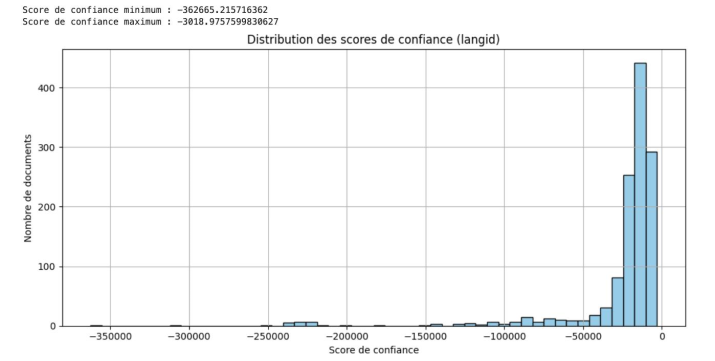
\includegraphics[width=.8\textwidth]{images/DescriptifConf.png}
  \caption{Que nous dit cette distribution ?}
\end{figure}
\end{frame}

\begin{frame}{Vérifier des propriétés des données : bonne idée}

\begin{figure}
  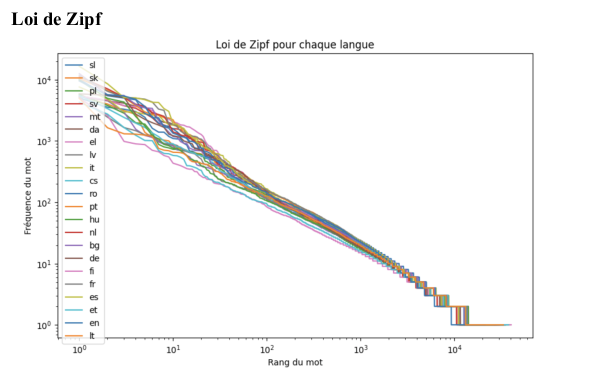
\includegraphics[width=.8\textwidth]{images/Zipf_muli.png}
  \caption{Que nous apprend cette courbe ?}
\end{figure}
\end{frame}

\section{Comparer des méthodes}

\begin{frame}{Interpréter les différences}

\begin{figure}
  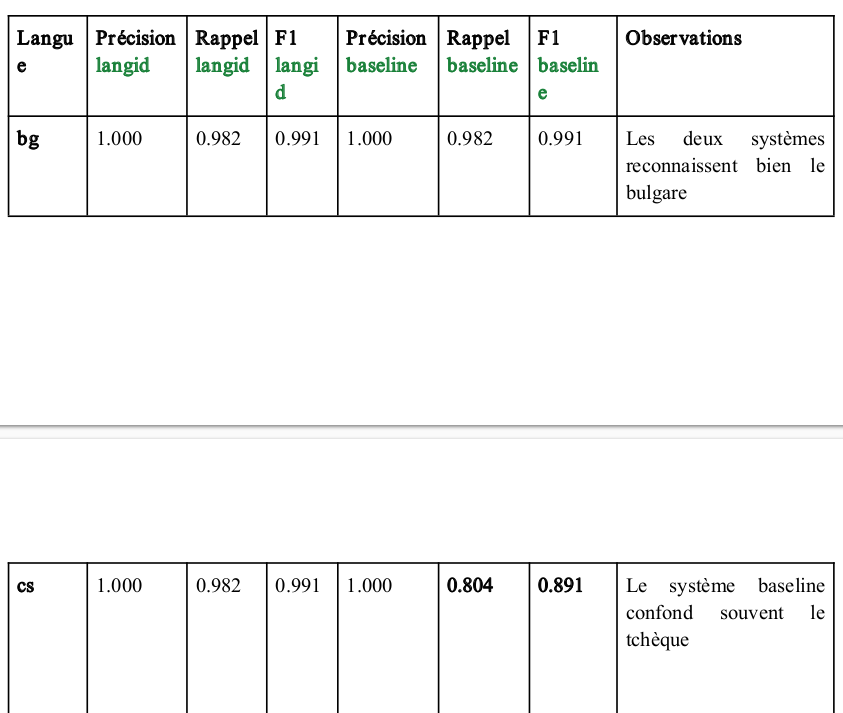
\includegraphics[width=.75\textwidth]{images/Quali.png}
  \caption{La comparaison par classe pour identifier des différences entre les méthodes}
\end{figure}
\end{frame}

\section{Observer des paramètres}

\begin{frame}{Mettre en perspective une évolution (I)}

\begin{figure}
  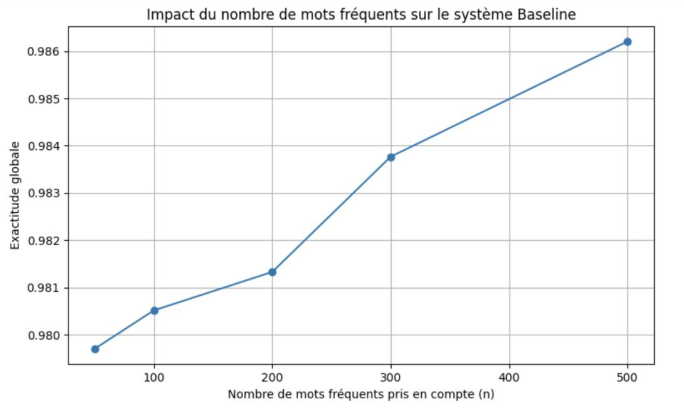
\includegraphics[width=.8\textwidth]{images/Scale2.png}
  \caption{Différence importante ou non ?}
\end{figure}

\end{frame}

\begin{frame}{Mettre en perspective une évolution (II)}

\begin{figure}
  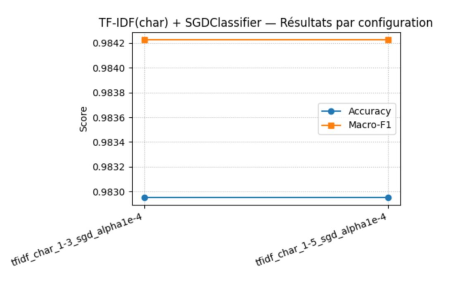
\includegraphics[width=.8\textwidth]{images/Scale3.png}
  \caption{Différence importante ou non ?}
\end{figure}

\end{frame}

\begin{frame}{Features}

\begin{figure}
  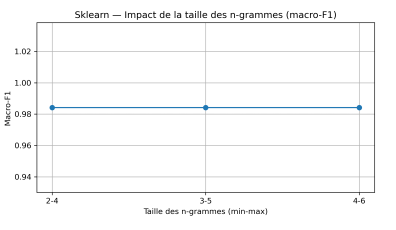
\includegraphics[width=1\textwidth]{images/Ngam_size.png}
  \caption{Comment interpréter l'absence de changement dans les résultats ?}
\end{figure}

\end{frame}

\begin{frame}{Interpréter une évolution}
\begin{figure}
  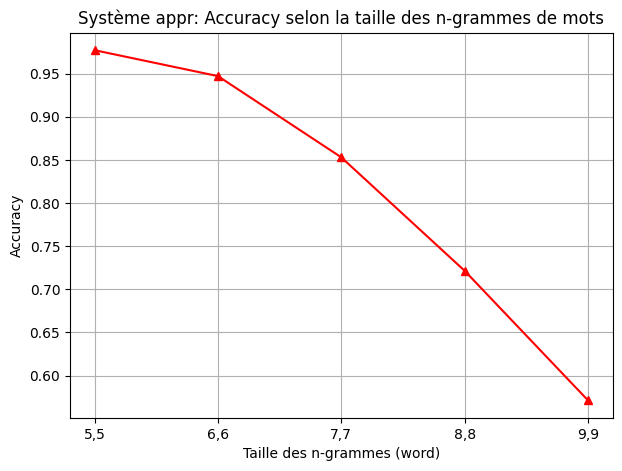
\includegraphics[width=1\textwidth]{images/Generalisation.png}
  \caption{Que se passe-t-il quand la taille des observables augmente ?}
\end{figure}

\end{frame}
\section{Prêter attention à l'échelle}


\begin{frame}{Micro VS Macro et échelle}

\begin{figure}
  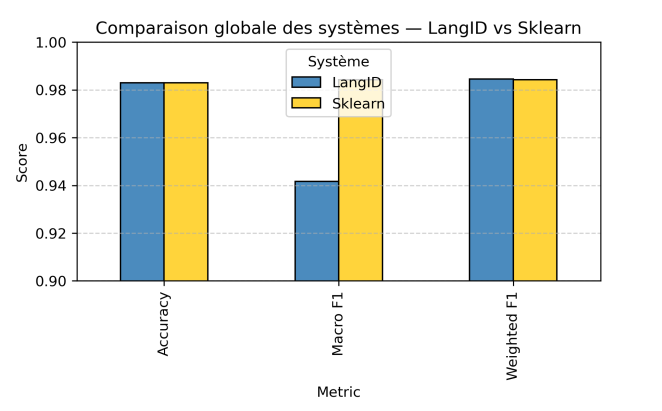
\includegraphics[width=1\textwidth]{images/Weighted_macro.png}
  \caption{Weighted VS Macro ?}
\end{figure}

\end{frame}
\begin{frame}{Heatmap : Quels usages}

\begin{figure}
  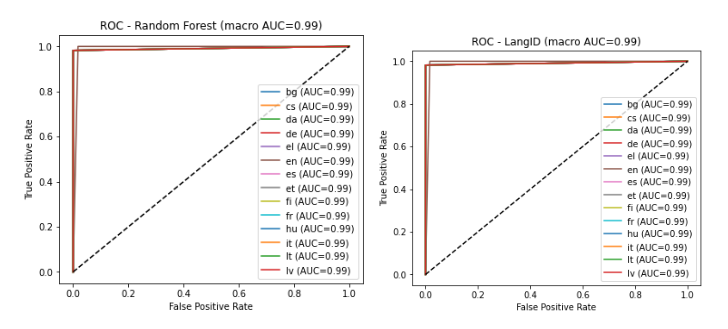
\includegraphics[width=.8\textwidth]{images/ROC_scale.png}
  \caption{Courbe ROC: valeurs et échelle}
\end{figure}

\end{frame}

\section{Détecter des bizarreries}
\begin{frame}{Lire des résultats (I)}

\begin{figure}
  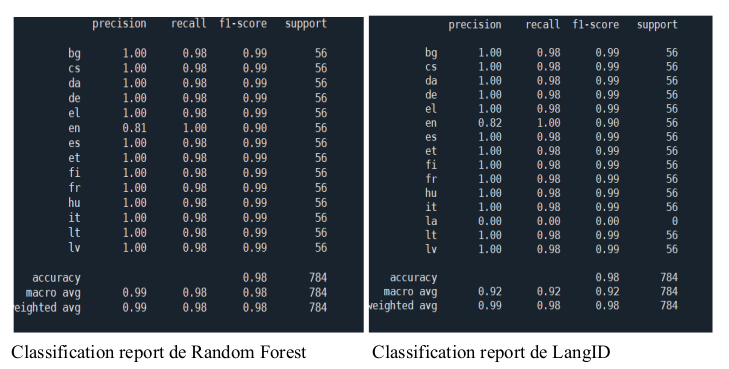
\includegraphics[width=1\textwidth]{images/Missing_classes.png}
  \caption{Comment détecter des résultats aberrants ?}
\end{figure}

\end{frame}

\begin{frame}{Lire des résultats (II)}

\begin{figure}
  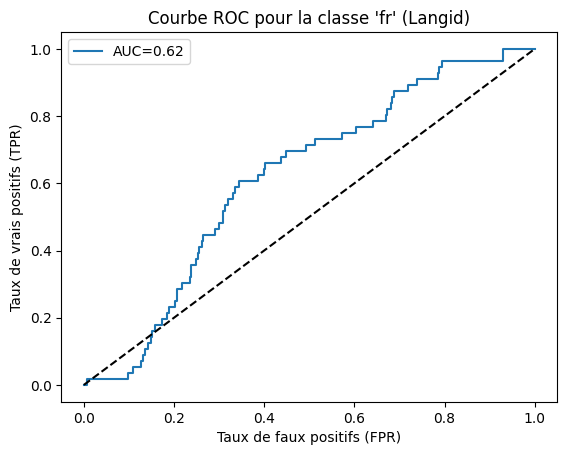
\includegraphics[width=.9\textwidth]{images/ROC_fail.png}
  \caption{Comment détecter des résultats étonnants ? Rapport Rappel bruit ?}
\end{figure}

\end{frame}

\begin{frame}{Lire des résultats (III)}

\begin{figure}
  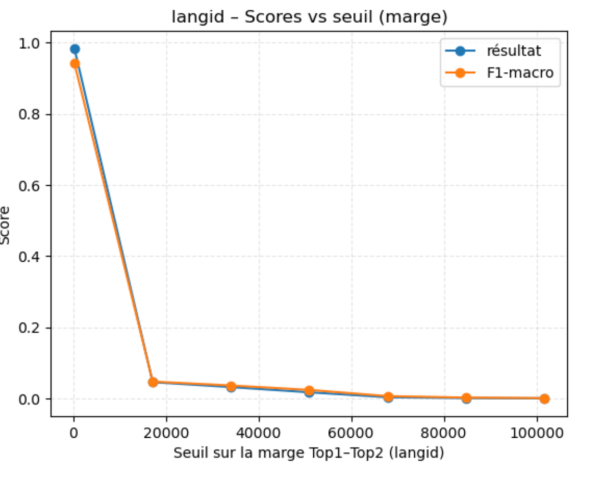
\includegraphics[width=1\textwidth]{images/Conf_Langid.png}
  \caption{Que signifie le score ?}
\end{figure}
%TODO: interpréter el score de langid
\end{frame}

\begin{frame}{Taux de Confiance  et gains possibles}

\begin{figure}
  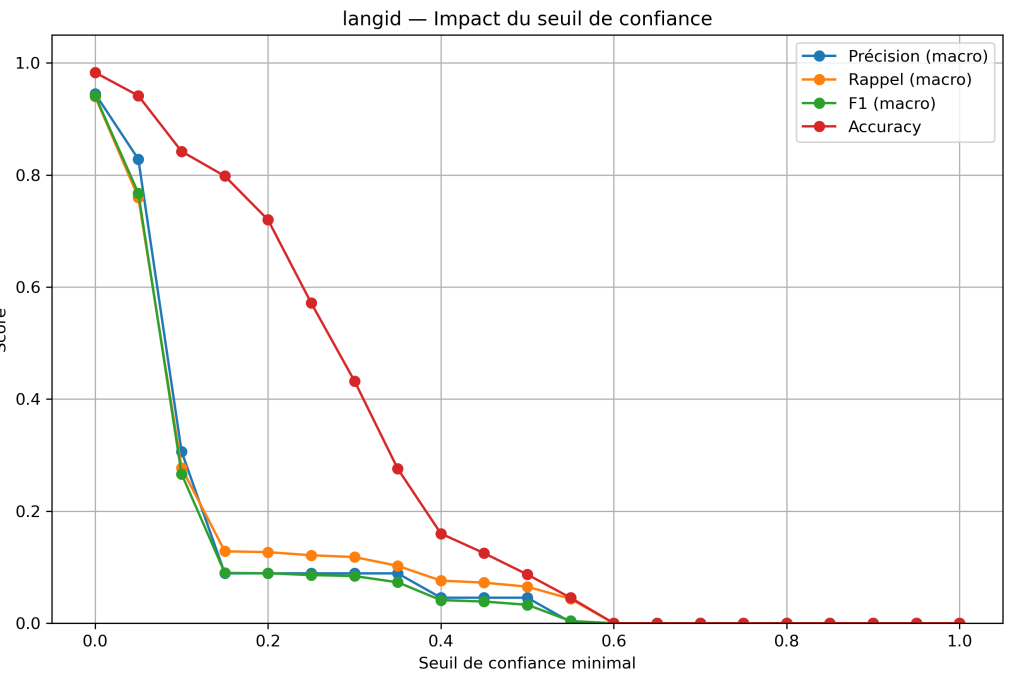
\includegraphics[width=1\textwidth]{images/TxConfiance.png}
  \caption{Pourquoi relever le taux de confiance n'améliore rien ?}
\end{figure}

\end{frame}

\begin{frame}{Seuil dans le "bon ordre" pour interpréter}

\begin{figure}
  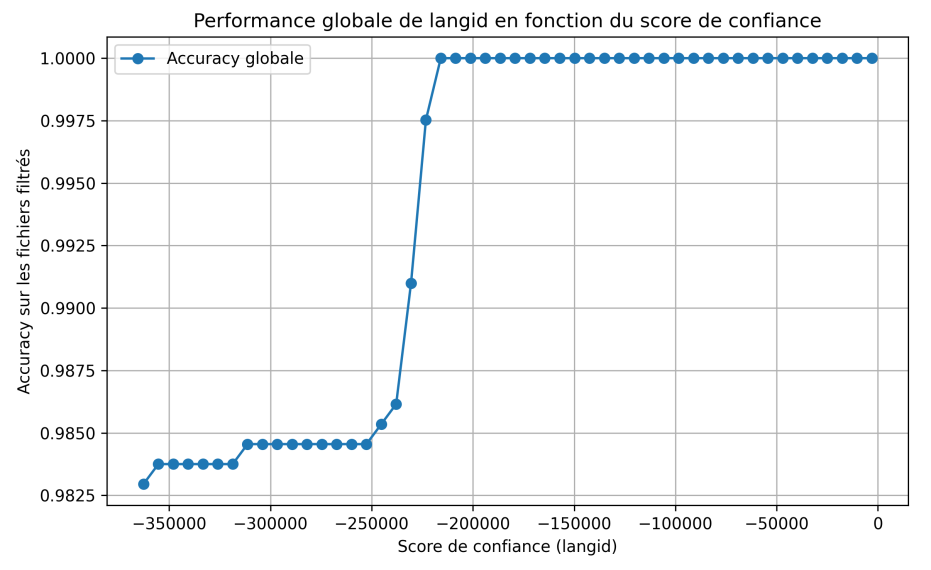
\includegraphics[width=1\textwidth]{images/ConfLangIdWorks.png}
  \caption{Propriétés attendues du taux de Confiance ?}
\end{figure}

\end{frame}


\section{Questionner les modes d'exposition des résultats}

\begin{frame}{Tableau ou Figure ?}

\begin{figure}
  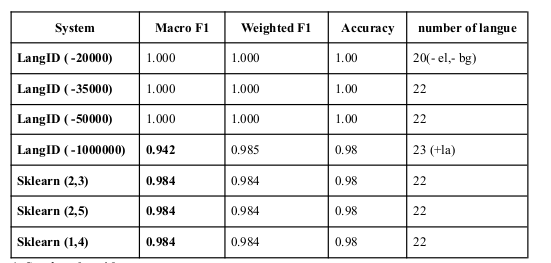
\includegraphics[width=1\textwidth]{images/TabVSFig.png}
  \caption{Limites de la présentation en tableau}
\end{figure}

\end{frame}

\begin{frame}{De la difficulté d'une tâche facile}
%TODO: scale
\begin{figure}%
\begin{subfigure}{0.45\textwidth}
\centering
  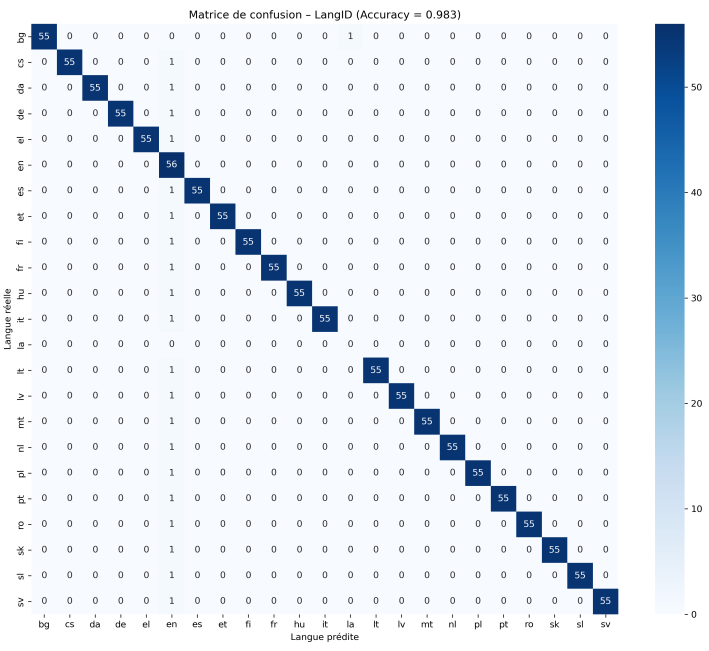
\includegraphics[width=1\textwidth]{images/HeatmapLangid.png}
  \caption{Système 1}
\end{subfigure}
\begin{subfigure}{0.45\textwidth}
  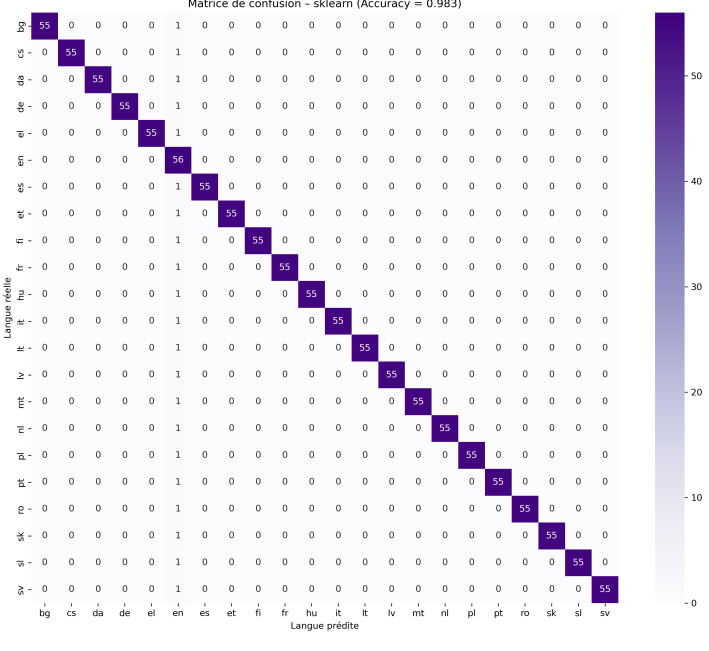
\includegraphics[width=1\textwidth]{images/HeatmapSkLearn.png}
  \caption{Système 2}
\end{subfigure}
\caption{Comment comparer ?}
\end{figure}

\end{frame}


\begin{frame}{La métrique ou la tâche}
\begin{figure}
  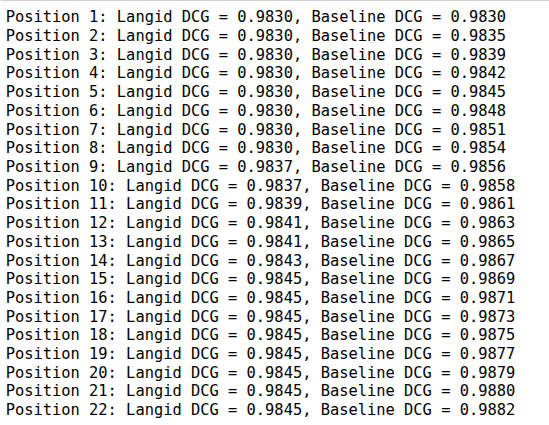
\includegraphics[width=.8\textwidth]{images/Rank_DCG.png}
  \caption{Pas d'évolution et donc ?}
\end{figure}

\end{frame}


\begin{frame}{Comment améliorer ?}
\begin{figure}
  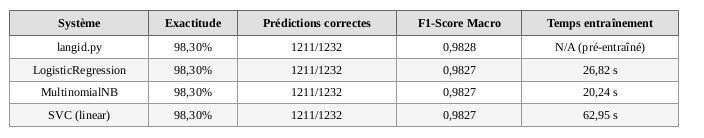
\includegraphics[width=1\textwidth]{images/CompClassifiers.png}
  \caption{Que peut-on faire de plus ?}
\end{figure}

\end{frame}

\section{Retourner aux données}

\begin{frame}{Quelles sont ces erreurs?}
\begin{figure}
  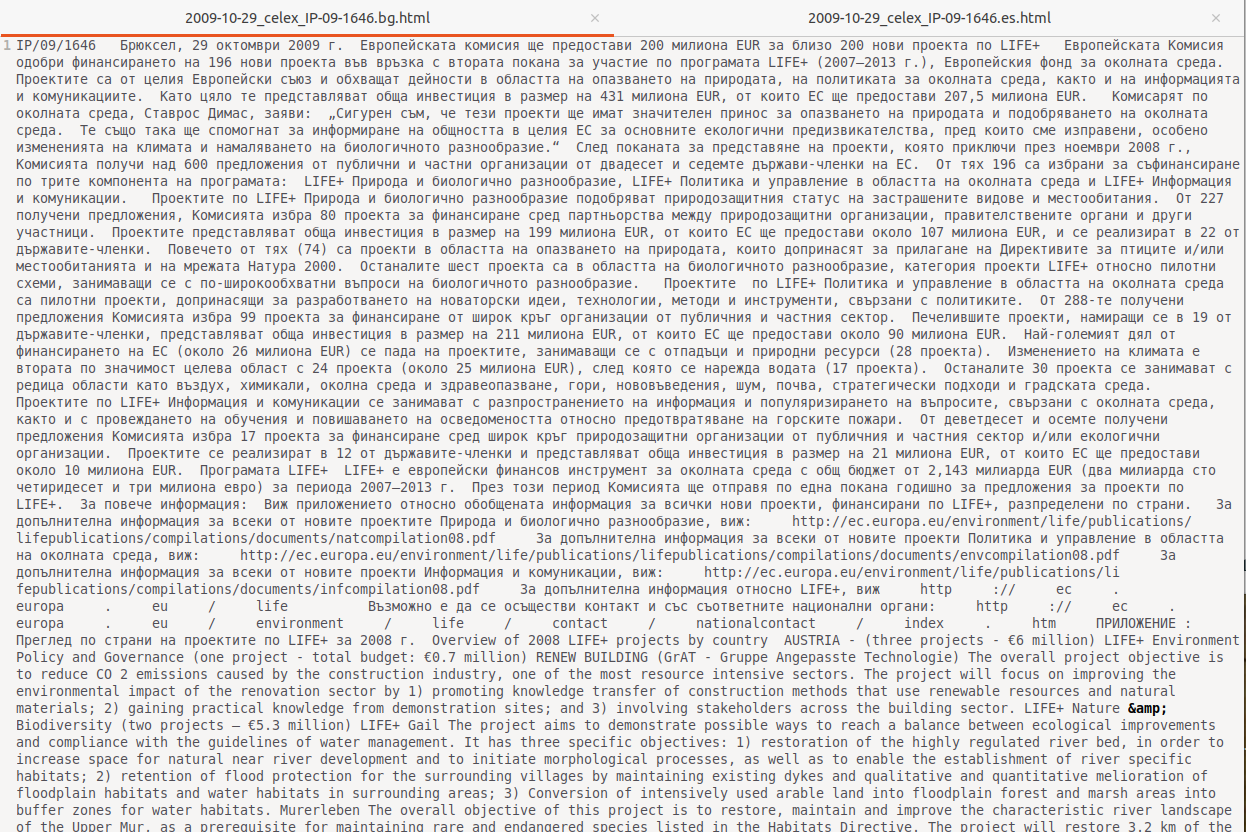
\includegraphics[width=1\textwidth]{images/Error_bg.png}
  \caption{Que peut bien signifier cette erreur récurrente? \texttt{bg/test/2009-10-29\_celex\_IP-09-1646.bg.html}}
\end{figure}

\end{frame}

\begin{frame}{Quelles sont ces erreurs?}
\begin{figure}
  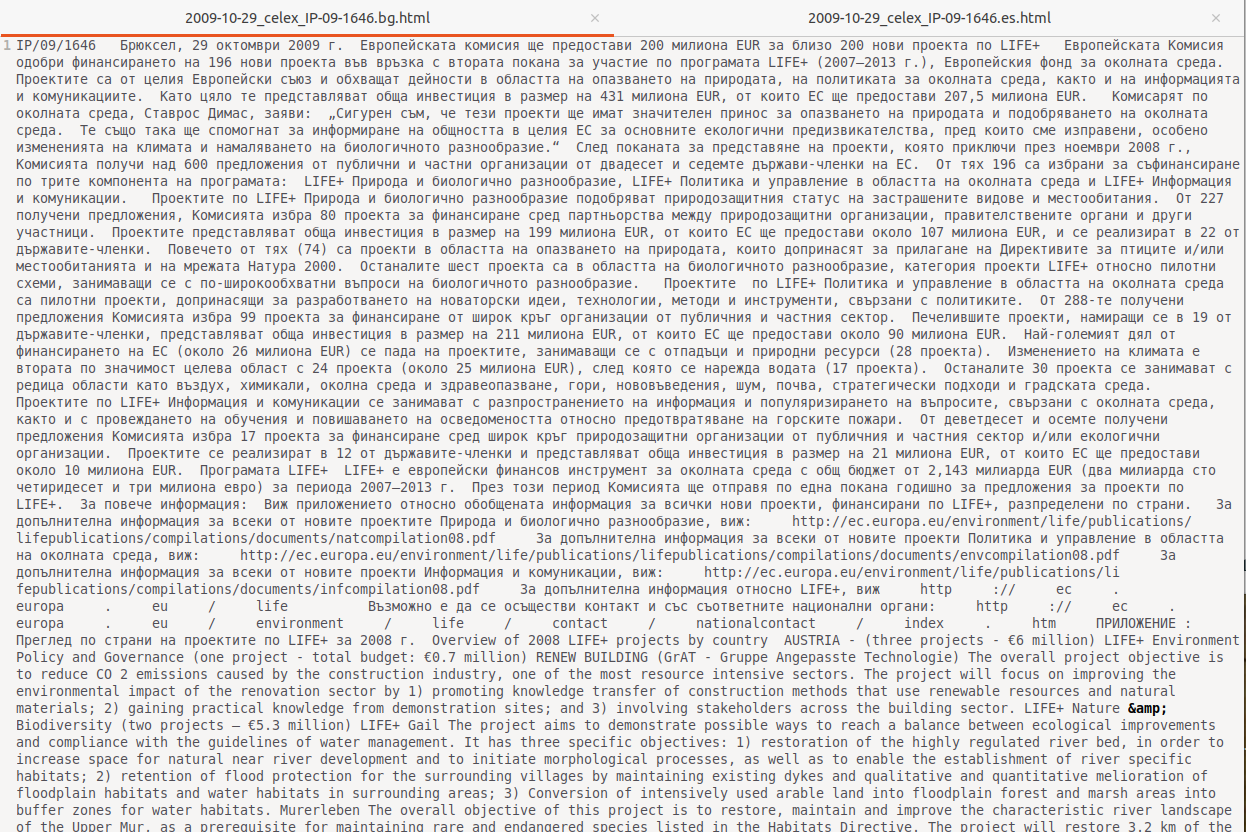
\includegraphics[width=1\textwidth]{images/Error_bg.png}
  \caption{Une erreur comparable en espagnol\dots \texttt{es/test/2009-10-29\_celex\_IP-09-1646.es.html}}
\end{figure}

\end{frame}

\begin{frame}{Travail pour dans 2 semaines}

Faire la même chose avec ce dataset de \textsc{Kaggle} : 

\url{https://www.kaggle.com/datasets/basilb2s/language-detection}

Rendu le 18/11 ?

\end{frame}


\end{document}
